
\section{Singapore --- Electronic Road Pricing (ERP)}

\subsection{Implementation}

While cheap to administer in a simple form, a manual system such as the Area License Scheme becomes intractable as pricing becomes more precise. For example, \citet[p. 4]{Chin2010} describes the functioning of ALS once multiple charging periods and vehicle classes were added: ``There were 16 different types of licences in use at its peak, and much concentration by the enforcement officers was required to ensure that they identified them correctly.''
To gain precision with less difficulty, in the early 1990s, Singapore solicited bids for an electronic system. The government chose a smart card/IU system like the one trialed in Cambridge, rather than a transponder system like the Hong Kong ERP, partly to alleviate privacy concerns \citep{PhangToh1997,Chin2010}. After extensive field trials and publicity, the electronic system---called, like Hong Kong's Electronic Road Pricing (ERP)---commenced operation in September 1998.

\subsection{Design}

\citet{Menon2004} describes ERP as having three components.

\begin{itemize}
\item In-vehicle Unit (IU), an electronic device that sits on vehicles' dashboards or handlebars and. The IU has a slot for a ``CashCard'' that the user can load up with money at various places.\footnote{The CashCard can also be used to pay for parking. In March 2015, a sevice called vCashCard was announced that allows drivers to pay with debit or credit without having a physical CashCard in the IU. (http://www.straitstimes.com/singapore/transport/virtual-cashcard-aims-to-solve-erp-woes)} There are IU's for each of six vehicle classes (see Figure \ref{fig:singapore-IUs}), because the toll charged to a vehicle is a multiple of its ``Passenger Car Unit'' (PCU), an index of how much roadspace the vehicle takes up (see Table \ref{tab:passenger-car-units}). 

\item Gantries (see Fig. \ref{fig:singapore-gantry}). Gantries are positioned in pairs. When a vehicle passes below, the first gantry signals the vehicle's IU, telling it to charge the CashCard appropriately. An optical sensor on the second gantry confirms the vehicle type matches the IU. In the event of error, a camera on the first gantry captures the rear number plate. 

\item The central control system, which verifies charges and issues notices and fines when there is a violation or error.
\end{itemize}

\begin{table}
	\begin{tabular}{|c|c|}
		\hline 
		PCU's & Vehicles\tabularnewline                              
		\hline 
		\hline 
		0.5   & motorcycles\tabularnewline                           
		\hline 
		1     & cars, taxis, light goods vehicles\tabularnewline     
		\hline 
		1.5   & heavy goods vehicles/small buses\tabularnewline      
		\hline 
		2     & very heavy goods vehicles/large buses\tabularnewline 
		\hline 
	\end{tabular}
	
	\caption{
	Passenger Car Units (PCU's) for ERP. Vehicle charges are weighted by the PCU number---e.g., a very heavy goods vehicle pays four times what a motorcycle does. \citep{LTA2016} 
	}
	\label{tab:passenger-car-units}
\end{table}

ERP varies tolls substantially by time-of-day. Figure \ref{fig:singapore-toll-schedule} illustrates a weekday toll schedule for the CBD cordon. For the first five years of ERP, tolls changed only at half-hour intervals. But since February 2003, whenever tolls change by more than S\$1, there is a five-minute interval in which tolls rise or fall by half the amount of the change, in order to discourage cars from slowing down or speeding up when tolls are about to change \citep{Menon2004}. The Land Transport Authority (LTA) of Singapore updates prices quarterly to maintain speeds of 45-65kph on expressways and 20-30 kph on roads in the RZ, because the LTA believes these speeds maximize flow \citep{Li1999}.
	
\begin{figure}
	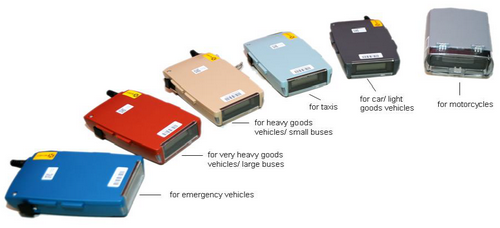
\includegraphics[width=4in]{../img/singapore-IUs.jpg}
	\caption{ERP In-vehicle units \citep{LTA2016}}
	\label{fig:singapore-IUs}
\end{figure}

\begin{figure}
	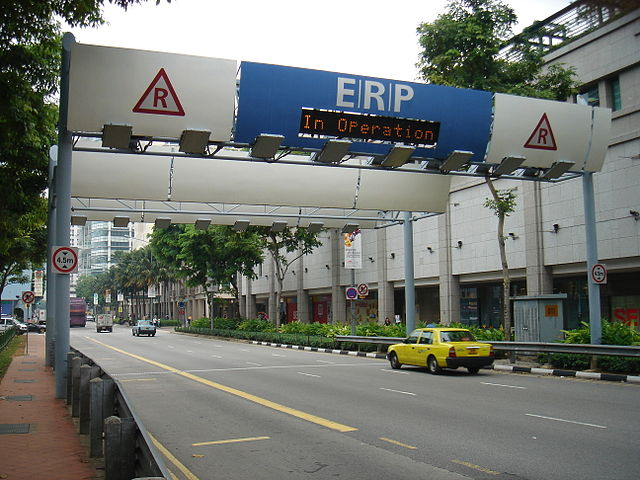
\includegraphics[width=4in]{../img/singapore-gantry.jpeg}
	\caption{ERP gantry \citep{LTA2016}}
	\label{fig:singapore-gantry}
\end{figure}


\begin{figure}
	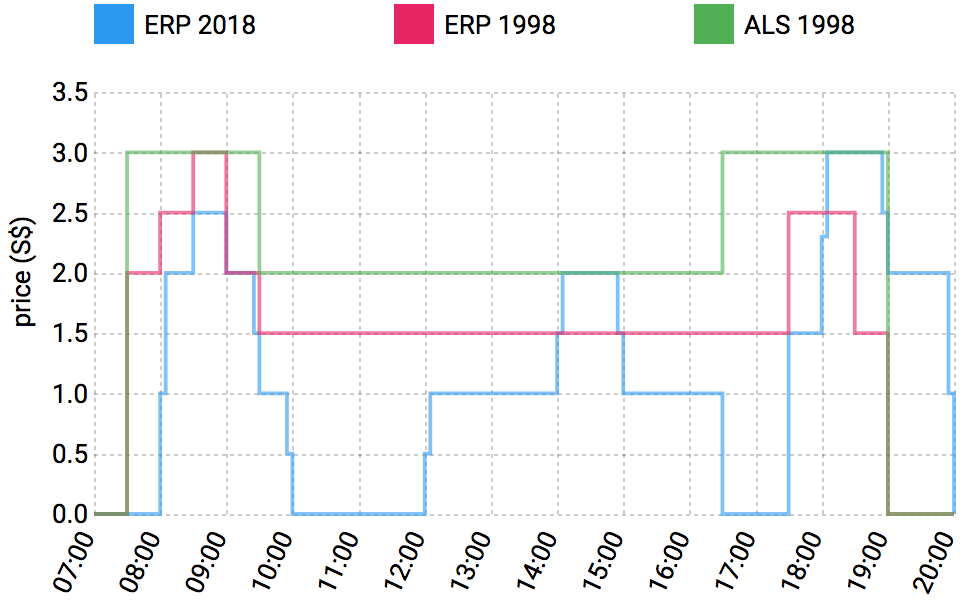
\includegraphics[width=5in]{../img/singapore-prices.png}
	\caption{Singapore prices for different years. The schedule becomes more variable as years pass. }
	\label{fig:singapore-toll-schedule}
\end{figure}

The substantial changes to the design of ERP have been spatial. ERP started in 1998 with 33 gantries that approximately reproduced the ALS cordon. Beginning in 1999, the LTA added gantries gradually to enclose the first cordon in a second ``Outer Cordon'' \citep{Chin2010}. In 2005, a shopping area on the border of the CBD Cordon became a sub-cordon called the Orchard Road Cordon, because shops open later than offices. The same year, gantries were added to charge outbound trips in the evening on one expressway. Finally, in 2008 a line of gantries was planted down the middle of the CBD Cordon. These operate only between 6 and 8PM, when intra-CBD congestion would otherwise be severe. By December 2014, ERP made use of 80 gantries \citep[p. 406]{Chu2015}.

\subsection{Results}

The transition to ERP was not as thoroughly documented as the launch of ALS. One significant effect is that entries to the CBD fell by about 15\%, largely due to a decline in repeat trips by the same vehicle \citep{Menon2000}. Since ALS permitted unlimited same-day entries, under ALS about 23\% of trips had been repeat trips---e.g., office workers using cars for lunches and meetings in the middle of the day \citep[p. 23]{Chin2010}. \citet{Olszewski2005} conclude, using data from before and after ERP, that the LTA's charging structure has done a good job controlling congestion and spreading traffic flow over the peaks.

\subsection{Finances}

ERP is unique among downtown pricing schemes in that its role as a source of revenue is negligible; the entire system is designed for congestion control, as government officials emphasize \citep{Chin2010}. Whereas the Area License Scheme and related Road Pricing Scheme together earned S\$9.3 million per month prior to the switch, ERP earned only S\$5.8 million per month, because ERP tolls were lower than an ALS license \citep[p. 34]{Goh2002}. Singapore does not regularly report revenues, but they were S\$159 million \citep{Chen2012}. ERP revenue is not hypothecated.

Implementation cost S\$197 million in 1998, of which S\$100 million paid for IU's (at a cost of S\$150 each) and S\$97 million to build out the infrastructure (e.g., to buy the gantries) \citep{Santos2004}. Annual operating costs have measured about 20-30 percent of revenues \citep{Chin2010}.